%%%%%%%%%%%%%%%%%%%%%%%%%%%%%%%%%%%%%%%%%%%
%  Header: Document Class, Packages, and New Commands
%%%%%%%%%%%%%%%%%%%%%%%%%%%%%%%%%%%%%%%%%%%

\documentclass{sig-alternate}
\usepackage{booktabs}
\usepackage[usenames,dvipsnames]{xcolor}
\usepackage[normalem]{ulem}
\usepackage{pifont}
\usepackage{multirow}
\newcommand{\urlwofont}[1]{\underline{\urlstyle{same}\url{#1}}}

\newif\ifrev
%  COMMENT OUT NEXT LINE TO HIDE TODOs AND COMMENTS
\revtrue

\ifrev
  \newcommand{\yanyan}[1]{{\color{blue} [Yanyan: #1]}}
  \newcommand{\cappos}[1]{{\color{red} [Justin: #1]}}
  \newcommand{\lois}[1]{{\color{magenta} [Lois: #1]}}
  \newcommand{\yiwen}[1]{{\color{OliveGreen} [Yiwen: #1]}}
  \newcommand{\todo}[1]{{\color{Orange} [TODO: #1]}}
\else
  \newcommand{\yanyan}[1]{}
  \newcommand{\cappos}[1]{}
  \newcommand{\linda}[1]{}
  \newcommand{\yiwen}[1]{}
  \newcommand{\todo}[1]{}
\fi

%%%%%%%%%%%%%%%%%%%%%%%%%%%%%%%%%%%%%%%%%%%
%  Begin of Document
%%%%%%%%%%%%%%%%%%%%%%%%%%%%%%%%%%%%%%%%%%%

\begin{document}

%%%%%%%%%%%%%%%%%%%%%%%%%%%%%%%%%%%%%%%%%%%
%  Title and Authors
%%%%%%%%%%%%%%%%%%%%%%%%%%%%%%%%%%%%%%%%%%%

\title{Quantifying and Minimizing the Risk of Kernel Exploitation}

\numberofauthors{5} 

\author{
% 1st. author
\alignauthor
Yiwen Li\\
       \affaddr{New York University}\\
       \email{liyiwen@nyu.edu}
% 2nd. author
\alignauthor
Ali Gholami\\
       \affaddr{KTH Royal Institute of Technology}\\
       \email{gholami@kth.se}
% 3rd. author
\alignauthor 
Christopher Matthews\\
       \affaddr{Apple Inc.}\\
       \email{chris4000@gmail.com}
\and
% 4th. author
\alignauthor
Yanyan Zhuang\\
       \affaddr{University of British Columbia}\\
       \affaddr{New York University}\\
       \email{yyzh@cs.ubc.ca}
% 5th. author
\alignauthor
Justin Cappos\\
       \affaddr{New York University}\\
       \email{jcappos@nyu.edu}
}

\maketitle

%%%%%%%%%%%%%%%%%%%%%%%%%%%%%%%%%%%%%%%%%%%
%  Abstract
%%%%%%%%%%%%%%%%%%%%%%%%%%%%%%%%%%%%%%%%%%%

\begin{abstract}

Securing privileged code (such as a kernel or hypervisor) is essential for
computer security.  Yet despite substantial effort, privileged code 
still contains exploitable vulnerabilities.  This has led to techniques
such as system call filtering, operating system virtualization, and library
OSes to allow secure computation of legacy code.  Unfortunately, these
techniques also exhibit exploitable vulnerabilities and do a poor job of 
preventing an attacker from exploiting flaws in the
underlying system.  In this paper, we analyze why existing techniques fail 
to protect the kernel effectively.  Moreover, to ground our
analysis, we devise a metric that allows us to predict which portions
of the kernel are less likely to contain vulnerabilities.
This metric is based upon whether lines of code in the kernel get 
executed by popular programs.  Our analysis shows that commonly used kernel 
paths contain fewer vulnerabilities.   

This observation has significant implications for how secure systems
should be designed.  As a result, we devised a novel ``safely-reimplement'' 
design pattern for secure systems.  We implemented a prototype security 
system Lind, that uses this design pattern.
%accesses only commonly used kernel paths, and have a very small trusted computing base that places only limited trust in the privileged code. 
Our experimental results show that programs run in Lind can trigger many
fewer vulnerabilities (X\%) versus existing systems like VirtualBox (XX\%),
Graphene (XX\%), and Bascule (XX\%).

\end{abstract}


%%%%%%%%%%%%%%%%%%%%%%%%%%%%%%%%%%%%%%%%%%%
%  Categories, Subject Descriptors, General Terms, and Keywords
%%%%%%%%%%%%%%%%%%%%%%%%%%%%%%%%%%%%%%%%%%%

\category{C.20}{General}{Security}
\category{D.4.6}{Security and Protection}{Security kernels}

\terms{Security, Measurement}

\keywords{Kernel Protection, Vulnerabilities, Sandbox}

%%%%%%%%%%%%%%%%%%%%%%%%%%%%%%%%%%%%%%%%%%%
%  Sections
%%%%%%%%%%%%%%%%%%%%%%%%%%%%%%%%%%%%%%%%%%%

\section{Introduction}
\label{sec.introduction}

\cappos{I talk about hypervisors too here, in part because I feel they are a
natural solution to the same problem.  I probably shouldn't because that makes
our scope seem larger than what we can support w/ our results.}

Privileged code \cappos{such as OS kernels and hypervisors} is an essential 
component of modern computer systems but 
presents a number of security challenges. The privileged code itself is vulnerable 
to attacks and other parts of the system could be damaged when vulnerabilities in 
that privileged code are exploited.

Failures in the trusted computing base (TCB) allow more impactful crashes, 
such as complete system failures, privilege escalation, etc. 
Decreasing the feasibility of exploitation of the kernel bugs, especially privilege escalation, 
would be a substantial step toward stronger security for computer systems.

Bugs in operating system kernels have motivated development of a diverse set of
technologies to attempt to reduce these risks, such as OS virtualization, 
system call filtering, library OSes, etc. \cappos{However, there are two
major problems with these systems.  First,}  Unfortunately, these technologies 
also harbor vulnerabilities that are also exploitable. \cappos{Second,}
Even with these technologies in place, applications from the user space 
could still have access to a portion of the kernel that might contain 
bugs and is risky to be exposed. 

One contributing factor to security problems associated with these existing technologies and potential
new designs is that it is still unknown which portions of the privileged code are
safe to expose, and which portions would be vulnerable and exploitable. 
One key missing puzzle is a standard method for quantifying the safety (or 
risk) of the privileged code. 
For example, is it a good practice to minimize \textit{the number of lines of code}?
Is \textit{the number of API calls} a good metric for security?  \cappos{cites
for these would be good.}
Is avoiding files that have historically had bugs a viable approach?
\cappos{Need to refer to the sorts of sources mentioned in this paper: 
``Does Bug Prediction Support Human Developers? Findings From a Google 
Case Study".  This refers to fairly close related work in the SE
community.  If mentioned here, it should be a sentence clause and a few
citations.  Section 3 can say more.}
To the best of our knowledge, there is no quantitative metric \cappos{that
is considered an effective way} to evaluate the 
security of privileged code \cappos{perhaps end the sentence here?  I feel
the rest gets away from what we want to say.} and provide 
insights into how to design a secure system that only interacts with the privileged code in a safe manner.

In this paper, we propose a metric that quantitatively measures and evaluated 
the \cappos{security of the Linux kernel versions X-Y}
kernel code. The kernel trace profiling data is an important piece of information 
obtained by using our metric. \cappos{I don't understand the previous sentence.
I think it may be clearer if rephrased.}
This data reveals the use pattern of the kernel code 
based upon applications running from the user space. The use pattern can then be
leveraged to design new systems that have to meet specific requirements, 
such as strong security or high performance. To design and build secure systems, 
a key hypothesis we have is that commonly used kernel paths contain few bugs, and are 
safe to be exposed. Results from using our metric indicate that this hypothesis is reasonable, and 
can be leveraged to create new design aiming at building secure systems. 

To protect the kernel from being exploited, we came up with a new design 
\cappos{do we want to name it here?  We should probably call it 
`safely-reimplement' so we can refer to it later.}
that aims at providing strong isolation between the kernel space and the user space, 
and thus providing better protection to the kernel. Our new design leverages 
our metric to make better design decisions and build more effective system. 
Based upon our new design, we implemented a sandbox system, called Lind.
Lind minimizes the amount of risky privileged code that is reachable by a
sandboxed program.  To allow a program that uses risky functionality to
execute correctly, risky functionality is reimplemented inside a sandbox with
a small trusted computing base (TCB) \cappos{comprised of safe code}. 
This additional level of sandboxing provides an outlet for risky functionality, without which
legacy programs will not run, while containing security flaws in this code. 

We evaluate Lind by comparing it against other similar systems 
that are not designed using our metric. More specifically, we run user applications
under Lind and other systems, and compare their kernel traces. In addition, we examined historical
kernel bug reports to verify whose kernel trace is likely to trigger more
kernel bugs. \cappos{I'm confused.  Do we use fuzzing or real apps for
this?}
Evaluation results showed that running applications in Lind is least likely to trigger kernel bugs, 
which indicates that designs, such as the prototype of Lind, which uses our metric, 
tend to result in more secure systems. 

The main contributions of this paper are as follows:

\begin{itemize}
\item We propose a novel metric for quantitatively measuring and evaluating 
the security of privileged code, such as in a hypervisor or kernel. 
Our metric examines the kernel trace generated by running popular user 
applications and produces recommendations at the lines-of-code level.  

\item Using our metric, we have findings that substantiated our key hypothesis that commonly used kernel paths 
contain few bugs.  \cappos{I wonder if this should be phrased differently.
Of course these results are things we found to be true.  If not, why would
we write the paper?  Do you want to say that we validated this on Linux
over certain versions of the kernel?}

\item We created a novel secure design paradigm `safely-reimplement' that 
came from examining and leveraging our metric and key hypothesis 
that commonly used kernel paths contain few bugs.  \cappos{Probably need a
sentence to describe it here.}
Using this new design, we implemented a sandbox we called Lind, which provides more secure environment
for running applications and provide strong protection to the kernel. 

\item Our evaluation results showed that implementation of our sandbox Lind did not trigger any of the 
zero-day vulnerabilities we examined, 
while systems built without using our metric have chances to trigger
\cappos{What does this mean?  It sounds like we don't know.} 
vulnerabilities, which suggests 
that our metric can help design and build more secure systems effectively.
\end{itemize}

The remainder of this paper is organized as follows. 
We discuss the motivation that drives our work in \S{2}. 
In \S{3}, we propose our metric as the solution to solve the problem and provide detailed discussion about the metric.
New architecture we designed using our metric is introduced in \S{4}. In \S{5}, we discuss the implementation of the design, a sandbox we called Lind. 
Evaluation results of our Lind system and the new design strategy are presented in \S{6}. 
We then discuss related work in \S{7} and conclude in \S{8}. 

\section{Motivation}
\label{sec.motivation}

The Operating System (OS) kernel is a critical component of the entire computing system, 
yet is not protected properly and very vulnerable under the current security model of existing 
computing systems.

The kernel has to provide an interface to serve the requests from user applications for acquiring 
essential system resources, such as memory, I/O, CPU, and etc. 
All applications running in the system depend on the kernel to provide 
essential functionality.   \cappos{Thus all code, even that which is 
sandboxed or untrusted, will make calls that are eventually processed by the
kernel.}

However, the OS kernel is privileged code that needs to be well protected. Access to the
kernel code should be avoided as much as possible and be conducted in a very careful manner 
whenever contact is necessary. Failing to do this would lead to potential exploitation of kernel bugs and 
may lead to serious damage to the entire computing system.  

\cappos{There is a shift in focus here.  We need to signal this somehow.}
The OS kernel has always been an appealing target. During the past few years, 
the exploitation of OS kernels has become a very serious problem that remains to be solved, 
in spite of large amount of efforts devoted by researchers and practitioners. 
There were 125 reported vulnerabilities of the Linux kernel, and 215 reported vulnerabilities 
of all kinds of kernels in 2014 \cite{NVD:14}. Admittedly, the exploitation of user-level software 
has become much harder, as recent versions of popular OSes come with numerous protections 
and exploit mitigations. The principle of least privilege is better enforced in user accounts 
and system services, compilers offer more protections against common software flaws, 
and highly targeted applications, such as browsers and document viewers, have started to 
employ sandboxing technique. On the other hand, the kernel has a huge codebase and 
an attack surface that keeps increasing due to the constant addition of 
new features \cite{Metrics:13}. Indicatively, the size of the Linux kernel in terms of lines of code 
has more than doubled, from 6.6 MLOC in v2.6.11 to 16.9 MLOC in v3.10 \cite{Linux:13}.

Opportunities for kernel exploitation are abundant. As an example consider the Linux kernel, 
which has been plagued by common software flaws, such as stack and heap buffer overflows 
\cappos{It seems like overkill to have all CVEs have their own cite.  Perhaps
just have one cite for the CVE system and then just list the number?}
\cite{CVE:20093234, CVE:20131828, CVE:20132892}, NULL pointer and pointer arithmetic errors 
\cite{CVE:20050736, CVE:20092698}, memory disclosure vulnerabilities 
\cite{CVE:20093002, CVE:20104073}, use-after-free and format string bugs 
\cite{CVE:20132852, CVE:20134343}, signedness errors \cite{CVE:20103437, CVE:20132094}, 
integer overflows \cite{CVE:20050736, CVE:20102959}, race conditions 
\cite{CVE:20091527, CVE:20093547}, as well as missing authorization checks and 
poor argument sanitization vulnerabilities 
\cite{CVE:20103904, CVE:20104347, CVE:20120946, CVE:20130268}. 
The exploitation of these bugs is particularly effective, 
despite the existence of kernel protection mechanisms, 
due to the weak separation between user and kernel space.
\cappos{What point are you trying to make with the last bit here?}

To build a secure computing system, it is critical to provide sufficient protection for the kernel and 
prevent kernel exploitation from happening. Many previous attempts, including OS virtualization, 
system call filtering, library OSes and etc. have tried to address this problem. However, 
kernel exploitation still exist, and the problem has not been solved 
effectively \cappos{This is a long sentence.  You may want to break it up.  }
\cappos{You also would be making a stronger point if you could support the claim
by showing flaws in those types of systems.}, which leads to a 
fundamental question, why is it not working and what are we missing? After thinking about this
question and examining previous work, we find that one key missing puzzle is that people do not know 
clearly which part of the kernel are safe and can be exposed without potential dangers. Many previous
work, such as building a sandbox and using library OSes focused on isolating user programs. While isolation 
can be useful and help mitigate the problem, the proposed systems still get access to the kernel. 
And the key is: the way they access the kernel has no difference than before, because they do not 
know what's the best way to leverage the kernel securely. So, essentially, what they are doing is just moving 
the attack surface from the previous place (between the user space and the kernel) to another place 
(between the new proposed system and the kernel). The attack surface
doesn't necessarily shrink.  \cappos{Is `shrinking' really the right thing
to consider?  I think we will argue against LOC as the metric.}
Therefore, the proposed solutions were not effective. 

It would be more effective, if we can actually shrink the attack surface and have better control over 
the interface exposed by the kernel. In another word, we need to be crystal clear about which portions of 
the kernel are safe and which portions of the kernel are risky.
\cappos{The previous sentence is a key point.  We need to draw it out and
justify it more.}  
\cappos{The text that follows feels like bridge text into the next section.
If so, it is much too long.  If you're trying to say what potential value
a metric would have, then you probably need to start a new paragraph and
make it clearer.  However, I think you talk about the value of the metric
in 3.1 as well, so you will likely want to combine text to avoid
duplication.}
To obtain this piece of critical information, we
propose a novel security metric to quantitatively measure and evaluate the kernel. Our metric will provide
insights into the kernel and let us understand security features of the kernel in a better way. 

With the help from our metric, we would be able to process the power of controlling the interface 
exposed to the user space in a precise and secure way. We can then design and build secure systems 
that provide stronger protection to the kernel. Ideally, we would like to only expose safe portion 
of the kernel to the user space. Realistically, in some cases, even if we have to expose certain risky portion 
of the kernel, we know clearly about the potential dangers and therefore can come up with better 
strategies to mitigate the potential damage. 

\section{A Quantitative Metric and Our Key Hypothesis}
\label{sec.metric}
We devised a metric to quantitatively evaluate security aspects of the kernel. 
It addresses a gap in that there is no standard method for properly evaluating 
a system's security level. Thus, enabling fair comparison to be made of different security tools. 
A critical question we investigated, using our metric is: which portions of the kernel are safe and 
contain few bugs? Our framing hypothesis is that \textbf{\textit{commonly used kernel paths}} contain few bugs. 
Our experimental results show that only $2.5\%$ of the historical kernel bugs that we examined were 
found in commonly used kernel paths. Based on this work, we created a new design, so that it 
places only limited trust within the commonly used kernel paths (in \S{4}). Using this new design, we built a prototype 
-- Lind -- as an example of how to use our metric to design and implement secure systems (in \S{5}). 

\begin{table*}[!ht]
\begin{tabular*}{\textwidth}{l @{\extracolsep{\fill}} lc}
\toprule
\multicolumn{3}{c}{Linux Kernel Bugs Examined} \\
\midrule
Vulnerability    &  Specific Type \\
\midrule
 CVE-2014-9529 \cite{CVE:20149529} & concurrency, race condition \\
 CVE-2014-3631 \cite{CVE:20143631} & NULL pointer dereference \\
 CVE-2012-6657 \cite{CVE:20126657} & network socket variable mischeck \\
 CVE-2014-5207 \cite{CVE:20145207} & privilege escalation \\
 CVE-2014-5206 \cite{CVE:20145206} & privilege escalation \\
 CVE-2014-3153 \cite{CVE:20143153} & privilege escalation \\
 CVE-2014-2851 \cite{CVE:20142851} & privilege escalation \\
 CVE-2014-2706 \cite{CVE:20142706} & race condition, DoS \\
 CVE-2014-0100 \cite{CVE:20140100} & race condition, DoS \\
 CVE-2014-0049 \cite{CVE:20140049} & buffer overflow \\
 CVE-2012-6638 \cite{CVE:20126638} & DoS \\
 CVE-2014-0038 \cite{CVE:20140038} & privilege escalation \\
 CVE-2013-6368 \cite{CVE:20136368} & privilege escalation  \\
 CVE-2013-4587 \cite{CVE:20134587} & index error, privilege escalation \\
 CVE-2013-4563 \cite{CVE:20134563} & size/boundary check, DoS \\
 CVE-2013-4348 \cite{CVE:20134348} & value validation error \\
 CVE-2013-4300 \cite{CVE:20134300} & privilege escalation  \\
 CVE-2013-1943 \cite{CVE:20131943} & privilege escalation \\
 CVE-2013-2094 \cite{CVE:20132094} & privilege escalation  \\
 CVE-2013-3301 \cite{CVE:20133301} & NULL pointer dereference, DoS \\
 CVE-2013-1858 \cite{CVE:20131858} & privilege escalation \\
 CVE-2013-1797 \cite{CVE:20131797} & use-after-free \\
 CVE-2013-1763 \cite{CVE:20131763} & privilege escalation, index error \\
 CVE-2013-0310 \cite{CVE:20130310} & NULL pointer dereference \\
 CVE-2012-2136 \cite{CVE:20122136} & heap-based buffer overflow \\
 CVE-2012-2100 \cite{CVE:20122100} & lack of sanity check \\
 CVE-2012-0028 \cite{CVE:20120028} & privilege escalation \\
 CVE-2011-2517 \cite{CVE:20112517} & privilege escalation, buffer overflow \\
 CVE-2012-2123 \cite{CVE:20122123} & privilege escalation \\
 CVE-2012-1146 \cite{CVE:20121146} & NULL pointer dereference \\
 CVE-2012-0207 \cite{CVE:20120207} & divide-by-zero error and panic \\
 CVE-2011-2525 \cite{CVE:20112525} & NULL pointer dereference \\
 CVE-2011-1076 \cite{CVE:20111076} & NULL pointer dereference \\
 CVE-2011-2184 \cite{CVE:20112184} & NULL pointer dereference, none Initialization \\
 CVE-2010-2478 \cite{CVE:20102478} & integer overflow \\
 CVE-2010-2960 \cite{CVE:20102960} & NULL pointer dereference  \\
 CVE-2010-2492 \cite{CVE:20102492} & privilege escalation, buffer overflow \\
 CVE-2010-2240 \cite{CVE:20102240} & stack overflow \\
 CVE-2010-1188 \cite{CVE:20101188} & use-after-free \\
 CVE-2010-0437 \cite{CVE:20100437} & NULL pointer dereference \\
\bottomrule
\end{tabular*}
\caption {Linux Kernel Bugs Examined}
\label{table:kernel_bugs}
\end{table*}

\subsection{Rationale Behind Our Metric}
As discussed previously (in \S{2}), a key reason that existing techniques 
fail to provide strong protection to the kernel is that there has yet to be a good way 
or standard method to understand which portions of the kernel are safe 
and which portions of the kernel are risky. We need to gain more knowledge to answer 
this question to properly decide how should the kernel be exposed to user applications, 
and what could be a good way to protect interactions between the kernel space and 
the user space, without drastic change to the current kernel structure. 
Thus, a metric to help solve this problem is desirable and could have huge practical impact. 

In addition to having a standard method for measuring and evaluating the kernel, 
our metric would also become a solid basis to conduct comparison between different tools that try to 
provide secure environment for running programs. 
Surprisingly, researchers and developers did not have a good way to evaluate the security features 
of their tools, let along conduct comparison between different tools. However, to achieve the 
goal of building and deploying secure systems, it would be very helpful if we could conduct fair and accurate 
comparison between different tools. Our metric provides a quantitative way to 
facilitate such comparison. An example of doing comparison for evaluating security features between different tools is 
demonstrated in our evaluation section (in \S{6}).

\subsection{How Does the Metric Work?}
To evaluate security aspects of the kernel using our metric, there are two key steps. First, 
\textbf{\textit{the kernel trace}} of which lines of code in the kernel get executed needs to be captured. 
Secondly, the kernel trace is checked against the historical kernel bugs to see if it contains kernel vulnerabilities. 

The first step in using our metric is to capture the lines of kernel code get executed. 
The Operating System kernel source code is organized under different kernel paths and folders. 
Whenever system resources, such as I/O, memory, and CPU, need to be accessed, the kernel code 
under corresponding paths will be executed to perform necessary functions. Therefore, the kernel code 
execution can be viewed as the fundamental activities of the kernel, and it reflects the basic behavior of 
the kernel. Thus, it makes sense to measure and analyze which lines of code get executed in the kernel. 
Our metric adopts this fundamental approach. It first captures which lines of code in the kernel get executed 
when running certain task programs, which we called the kernel trace. The kernel trace closely
ties with the set of task programs that generated the trace. Therefore, conducting comparison between 
different tools and environments becomes possible by using the kernel traces. To capture the kernel trace, 
we used a tool called Gcov \yiwen{cite: Gcov}, which is a component inside the Linux kernel.

The next step is to evaluate security aspects of the kernel trace that we captured. Using the historical kernel vulnerability 
reports, we built a list of severe kernel bugs. For each of the bugs we examined, we identified the lines of code 
in the kernel that would trigger the bug. We determine that the lines of code in the kernel are \textit{risky} if they 
may trigger certain kernel vulnerabilities. And those lines of code that cannot trigger kernel vulnerabilities are 
considered to be \textit{safe}. This gives us a precise way to know which portions of the kernel are safe and which 
portions of the kernel are risky. 

\subsection{Key Hypothesis: Commonly Used Kernel Paths Contain Few Bugs}
Now, to address the problem that motivated our metric from the very beginning, which portions of the kernel 
are safe and which portions of the kernel are risky. We can use our metric to answer this question. To be more
specific, we use our metric to get an idea of which lines of code in the kernel contain few bugs, then label 
those lines as safe lines. The safe lines of code would then compose the safe portions of the kernel, which can 
be trusted to build a secure trusted computing base for designs of secure systems (shown in \S{4}). 

Our hypothesis is that commonly used kernel paths are likely to be safe and contain few bugs. 
Here, ``commonly used kernel paths'' refers to the kernel paths executed by running popular and 
daily-used applications, such as Web browser applications, file editor applications, and etc. 
The logic behind our hypothesis is that commonly used kernel paths are used frequently, usually 
on a daily basis, and therefore have been well examined and reinforced by the security community and
the kernel development teams. In addition, commonly used kernel paths usually include 
kernel functions that are used in a normal way rather than special corner cases, which means that the chances 
to harbor kernel bugs in those commonly used kernel paths are slim. 

If our hypothesis can be verified, then it would become a critical guideline to create new designs for secure systems 
(shown in \S{4}). 
But before going too far into the new designs, let us first verify that our hypothesis indeed holds, that 
commonly used kernel paths are likely to contain few bugs and be safe. 

\subsection{Verification of the Key Hypothesis}
Our hypothesis is that commonly used kernel paths contain few bugs. 
So to verify our hypothesis, we first needed to obtain the commonly used kernel paths. 
We generated the commonly used kernel paths by using and combining two approaches, 
system call fuzzing, and running popular user applications. 

User space applications interact with the kernel space essentially through the system call API. 
So all those system calls are at the bottom level, while the applications sit at the top level. 
It makes sense then to obtain the kernel trace from both of those two different levels. 
We used two different approaches to obtain the kernel trace of commonly used kernel paths. 
Experiments of both approaches were conducted using the Native Linux environment.

\textbf{1) the bottom-up approach: system call fuzzing.}
Our system call fuzzing is basically running system calls exhaustively with all possible 
arguments and options. We conducted system call fuzzing over more than 300 available system calls, 
which gave us a thorough kernel trace. 

\textbf{2) the top-down approach: running popular user applications.} 
We ran applications that are commonly used by many users on a daily basis, such as Web browser application
and file editor application.  

\begin{table}[ht]
\centering
\begin{tabular}{|l|c|}
  \hline
  Approach & Kernel Coverage (percentage) \\
  \hline \hline
  System Call Fuzzing & 23\% \\
  \hline
  User Applications & 19\% \\
  \hline
\end{tabular}
\caption {Kernel Coverage}
\label{table:kernel_coverage}
\end{table}

\begin{figure}[h]
\centering
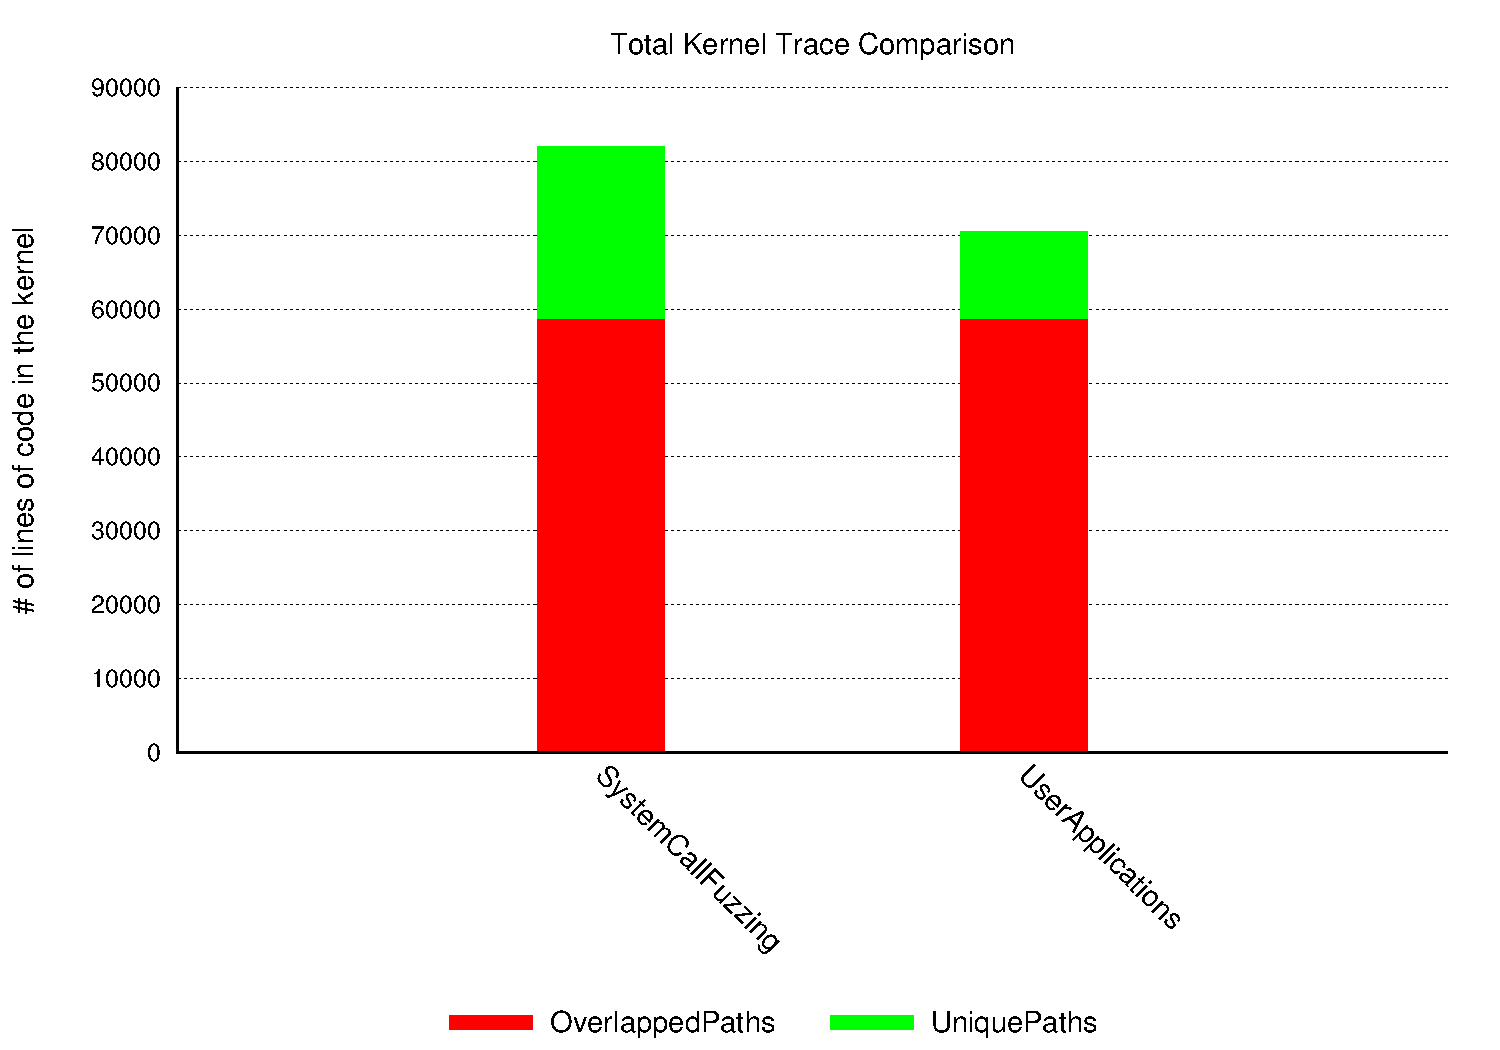
\includegraphics[width=1.0\columnwidth]{diagram/lind_ccs15_diagram_01.pdf}
\caption{Kernel Trace Comparison: Two Approaches}
\label{fig:two_approaches_trace}
\end{figure}

\begin{figure}[h]
\centering
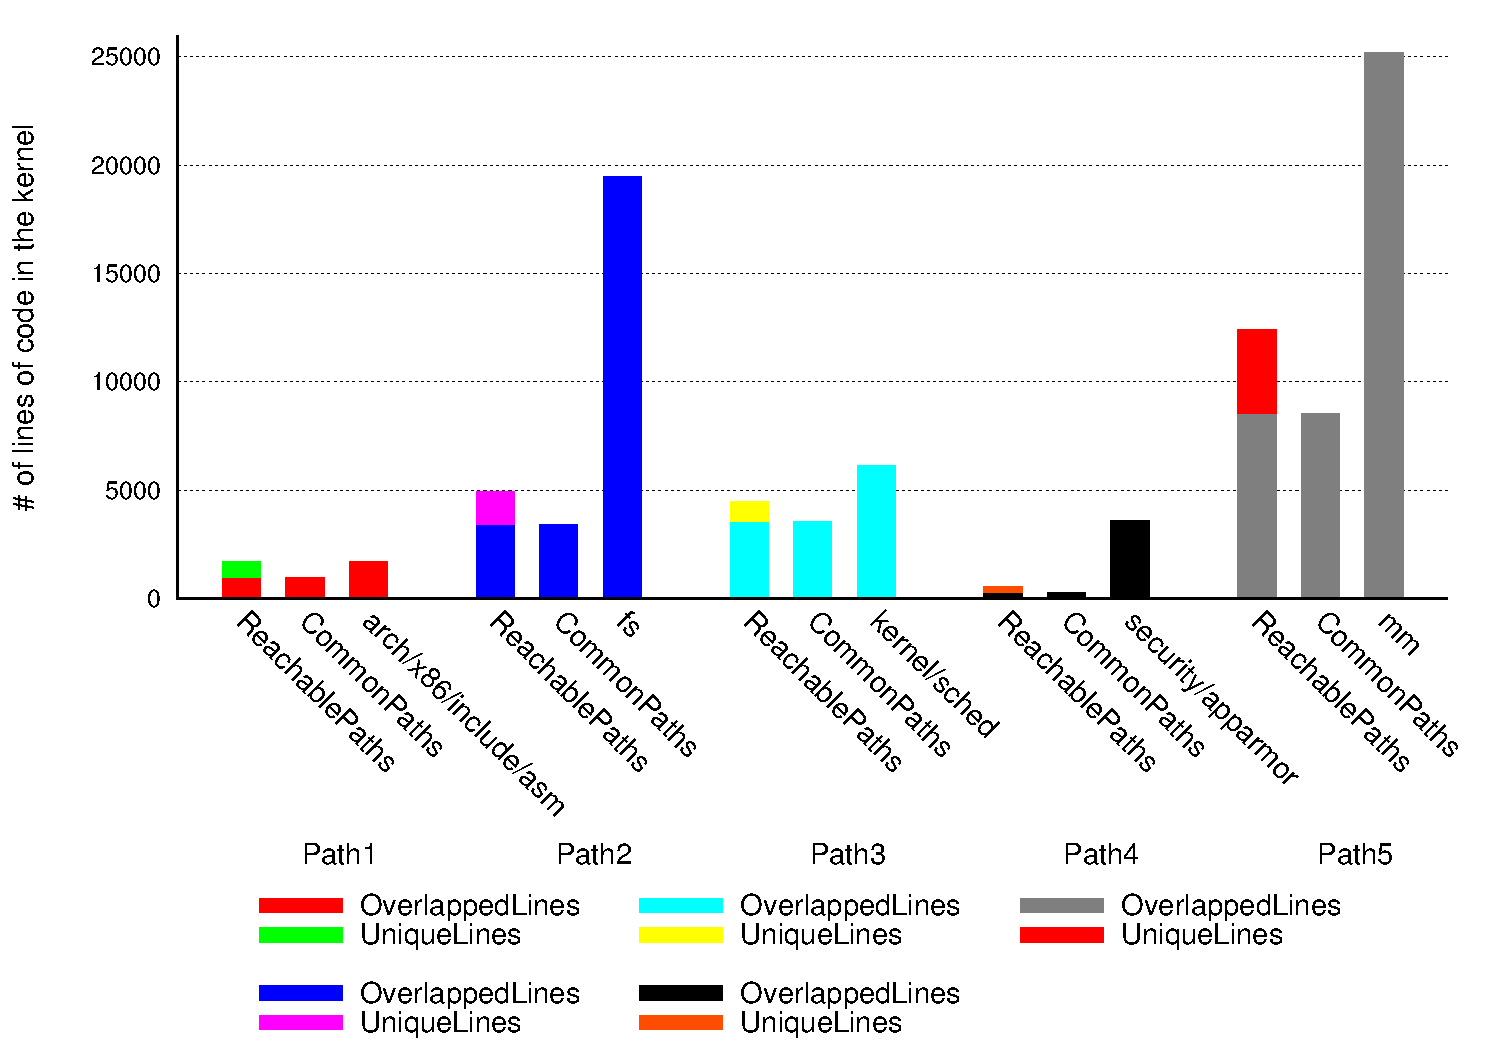
\includegraphics[width=1.0\columnwidth]{diagram/lind_ccs15_diagram_02.pdf}
\caption{Kernel Trace in Key Paths}
\label{fig:key_paths_trace}
\end{figure}

\begin{table*}[!ht]
\begin{tabular*}{\textwidth}{l @{\extracolsep{\fill}} cc}
\toprule
\multicolumn{3}{c}{Vulnerabilities in Commonly Used Kernel Paths} \\
\midrule
& \multicolumn{2}{c}{Commonly Used Kernel Paths} \\
\cline{2-3}
Vulnerability    &  System Call Fuzzing Paths &  User Application Paths \\
\midrule
 CVE-2014-9529 \cite{CVE:20149529} & \ding{55} & \ding{55} \\
 CVE-2014-3631 \cite{CVE:20143631} & \ding{55} & \ding{55} \\
 CVE-2012-6657 \cite{CVE:20126657} & \ding{55} & \ding{55} \\
 CVE-2014-5207 \cite{CVE:20145207} & \ding{55} & \ding{55} \\
 CVE-2014-5206 \cite{CVE:20145206} & \ding{55} & \ding{55} \\
 CVE-2014-3153 \cite{CVE:20143153} & \ding{55} & \ding{55} \\
 CVE-2014-2851 \cite{CVE:20142851} & \ding{55} & \ding{55} \\
 CVE-2014-2706 \cite{CVE:20142706} & \ding{55} & \ding{55} \\
 CVE-2014-0100 \cite{CVE:20140100} & \ding{55} & \ding{55} \\
 CVE-2014-0049 \cite{CVE:20140049} & \ding{55} & \ding{55} \\
 CVE-2012-6638 \cite{CVE:20126638} & \ding{55} & \ding{55} \\
 CVE-2014-0038 \cite{CVE:20140038} & \ding{55} & \ding{55} \\
 CVE-2013-6368 \cite{CVE:20136368} & \ding{55} & \ding{55} \\
 CVE-2013-4587 \cite{CVE:20134587} & \ding{55} & \ding{55} \\
 CVE-2013-4563 \cite{CVE:20134563} & \ding{55} & \ding{55} \\
 CVE-2013-4348 \cite{CVE:20134348} & \ding{55} & \ding{55} \\
 CVE-2013-4300 \cite{CVE:20134300} & \ding{55} & \ding{55} \\
 CVE-2013-1943 \cite{CVE:20131943} & \ding{55} & \ding{55} \\
 CVE-2013-2094 \cite{CVE:20132094} & \ding{55} & \ding{55} \\
 CVE-2013-3301 \cite{CVE:20133301} & \ding{55} & \ding{55} \\
 CVE-2013-1858 \cite{CVE:20131858} & \ding{55} & \ding{55} \\
 CVE-2013-1797 \cite{CVE:20131797} & \ding{55} & \ding{55} \\
 CVE-2013-1763 \cite{CVE:20131763} & \ding{55} & \ding{55} \\
 CVE-2013-0310 \cite{CVE:20130310} & \ding{55} & \ding{55} \\
 CVE-2012-2136 \cite{CVE:20122136} & \ding{55} & \ding{55} \\
 CVE-2012-2100 \cite{CVE:20122100} & \ding{55} & \ding{55} \\
 CVE-2012-0028 \cite{CVE:20120028} & \ding{55} & \ding{55} \\
 CVE-2011-2517 \cite{CVE:20112517} & \ding{55} & \ding{55} \\
 CVE-2012-2123 \cite{CVE:20122123} & \ding{55} & \ding{55} \\
 CVE-2012-1146 \cite{CVE:20121146} & \ding{55} & \ding{55} \\
 CVE-2012-0207 \cite{CVE:20120207} & \ding{55} & \ding{55} \\
 CVE-2011-2525 \cite{CVE:20112525} & \ding{55} & \ding{55} \\
 CVE-2011-1076 \cite{CVE:20111076} & \ding{55} & \ding{55} \\
 CVE-2011-2184 \cite{CVE:20112184} & \ding{55} & \ding{55} \\
 CVE-2010-2478 \cite{CVE:20102478} & \ding{55} & \ding{55} \\
 CVE-2010-2960 \cite{CVE:20102960} & \ding{55} & \ding{55} \\
 CVE-2010-2492 \cite{CVE:20102492} & \ding{55} & \ding{55} \\
 CVE-2010-2240 \cite{CVE:20102240} & {\color{red}\ding{51}} & {\color{red}\ding{51}}\\
 CVE-2010-1188 \cite{CVE:20101188} & \ding{55} & \ding{55} \\
 CVE-2010-0437 \cite{CVE:20100437} & \ding{55} & \ding{55} \\ 
\bottomrule
\end{tabular*}
\caption {Vulnerabilities in Commonly Used Kernel Paths 
({\color{red}\ding{51}}: vulnerability in paths; \ding{55}: vulnerability not in paths)}
\label{table:vulnerabilities_commonly_used_kernel_paths}
\end{table*}

Using the two approaches we just described, we obtained the trace of commonly used kernel paths.
The kernel trace coverage of the two approaches are as shown in Table 2. 
A further breakdown of the composition of the kernel trace is illustrated in Figure 1 and Figure 2.

The results from Table 2 show that the size of commonly used kernel paths is not very large, only about $20\%$ 
of the entire kernel code base. This is a positive sign that shows that commonly used kernel paths are likely to contain 
few bugs, since the coverage of the commonly used kernel paths is small and leaves little space for vulnerabilities to exist. 

The results from Figure 1 and Figure 2 show that for the two different approaches we used, most of the kernel trace was shared 
and under common paths. 
(Shown by the ``OverlappedPaths'' from Figure 1 and ``OverlappedLines'' from Figure 2.) 
This shows that the kernel trace we generated was indeed commonly used, 
so our method to obtain commonly used kernel paths is reasonable. 

We then checked if those commonly used kernel paths contain few kernel bugs.
We examined a list of 40 severe Linux kernel bugs from the last five years (shown in Table 1). 
We used those 40 kernel bugs to check if there are vulnerabilities within the trace of commonly used kernel paths.
The results of our experiment are shown in Table 3.  

From the results, we can see that commonly used kernel paths contain only $2.5\%$ of the bugs we examined 
from the last five years.  
Our results have positive implication that commonly used kernel paths contain few bugs and are safe. 
Our hypothesis and finding provide insights and guidelines for new designs of secure systems. We discuss details of 
a new design in the next section, \S{4}. 
\section{A New Design for Building Secure Systems}
\label{sec.design}

Our goal is to build secure systems that can mitigate the problem of kernel exploitation effectively. 
As we have discussed in the motivation section \S{2} before, one key reason that many previous work 
failed to prevent kernel exploitation effectively is that there was not enough knowledge about 
which portions of the kernel can be safely exposed to the user applications. 
And there was no standard method to acquire this knowledge. 
The metric we introduced in \S{3} is devised to serve the purpose of having a standard method to 
obtain better understanding of the kernel, and to know which portions of the kernel can be safely exposed. 
As we discussed in \S{3}, our findings suggest that commonly used kernel paths contain few bugs.
We shall then use this important result to create a new design for building secure systems. 

\subsection{Threat Model}
In our threat model, threats refer to any behavior, either intentional or accidental, that may cause potential harm 
to the system. Threats may be triggered by malicious code or bugs in non-malicious programs.

In order to fully execute their functions, applications need to have access to a set of privileges provided by 
the operating system, usually exposed as system calls. The primary security goal of a secure system is to 
restrict a program to some subset of privileges, usually by exposing a set of functions that mediate 
access to the underlying operating system privileges. Threats occur when applications obtain access to 
privileges that were not intentionally exposed by the system, thus escaping the protection 
intended by the secure system \cite{Repy:10}.

To pose threats to a secure system, we assume that applications may use multiple threads to modify visible 
state or issue concurrent requests which may trigger a race condition. Our goal is to prevent bugs in 
the code from allowing an user program to escape the secure system to access the kernel code, and 
possibly trigger kernel bugs.

\subsection{Design of Architecture}
To build secure systems, our design needs to effectively construct a safe environment in which user programs 
can run without worrying about triggering kernel bugs and break the whole system. To achieve this security goal, 
our secure system should be placed in the user space, and exist as a key layer between the user applications 
and the underlying Operating System kernel. To complete the architecture of the system, there are three critical 
questions that need to be answered. First of all, how should our system access the kernel? Secondly, what interface 
should our system provide to the user programs? Finally, how to implement the inside of our system to make it work?

To begin with, the key question related with security is how should our system access the kernel. Since now we know 
that commonly used kernel paths contain few bugs, it would be desirable to design a system that only access the 
commonly used kernel paths. Through our findings in \S{3}, we can see that commonly used kernel paths have relatively 
small size. This is positive for our design, because it shows that it is possible to design a system with a very small 
trusted computing base. Thus, our design should only access fundamental system calls within commonly used kernel paths. 
This gives our design a very small trusted computing base that places only very limited trust in the kernel code. Therefore, 
our design barely has the chance to trigger kernel bugs and cause serious security problems. 

Next, what interface should our system provide to the user programs? Essentially, this represents the tradeoff between 
security and functionality. Our goal is to provide strong protection to our system, therefore, security is prioritized. We are willing 
to sacrifice certain functionality if better security can be achieved. Thus, our design provides a POSIX API to user programs with 
support of fundamental functions. In fact, a restricted POSIX API is good enough to support many popular applications, 
and even some very complex legacy applications. 

Finally, how to implement the inside of our systems? 
To provide a rich POSIX API to user programs, while accessing the kernel only in commonly used path requires our system to 
reconstruct and reimplement many functions inside our system. Since the reimplementation itself is hard and may contain bugs 
and raise security concerns, in our design, we require the reimplementation to be done inside a sandbox. Within a contained 
environment, the reimplementation can construct the POSIX API effectively, without worrying about break other parts of the system.  

\subsection{Conclusion}
We have shown that using our finding that commonly used kernel paths contain few bugs as a key principle, a new design was created 
for building secure systems. Our design accesses only commonly used kernel paths, placing very limited trust within the kernel code. 
To provide sufficient functionality to user programs, our design safely reimplement fundamental functions inside a sandbox. Thus, many 
popular user applications and legacy programs can be supported by the POSIX API our system provides, while security will not be violated 
with the isolation provided by the sandbox. 

The design we described here doesn't rely on any specific technique or tool. To implement our design, it is possible to choose different techniques 
that suit well with specific needs or requirements. In the next section (\S{5}), we describe one implementation we did using our design. 
\section{Implementation}
\label{sec.implementation}

Based on the new design we introduced in \S{4}, we implement a secure system, called Lind, as 
as test and verification for our new design and the metric we used behind the design. We discuss 
implementation details of our system Lind in this section. 

\subsection{Two Basic Techniques: Google's Native Client and Repy Sandbox}
In the implementation of Lind, we leveraged two existing technologies, Google's Native Client, 
and Repy sandbox. We now give a brief introduction to those two technologies.
\cappos{Perhaps briefly state our reason for selecting each before explaining 
their details.}

Google's Native Client (NaCl) is a sandbox for untrusted x86 native code \cite{NaCl:09}. 
NaCl aims to give applications the computational performance of native applications 
without compromising safety. NaCl uses software fault isolation 
and a secure runtime to direct system interaction and side effects through interfaces managed by NaCl. 
NaCl provides operating system portability for binary code 
while supporting performance-oriented features, 
such as thread support, instruction set extensions such as SSE, and use of compiler intrinsics and 
hand-coded assembler. We leverage NaCl execution environment. NaCl allows the efficient execution of legacy code 
in the form of x86 and ARM binaries that are built with a lightly modified compiler tool chain.

Repy is a restricted subset of Python \cite{Repy:10}, which is a sandbox that 
provides safe environment for running applications.

In Lind, we use Repy to safely re-implement a subset of the POSIX API, which provides 
fundamental operating system access to many applications. The POSIX API, which itself is difficult to secure, 
is constructed using the Seattle's Repy sandbox which provides performance isolation and safety. 

It should be noted that those two techniques, Google's Native Client and Repy Sandbox, are not required
our new secure design. It is possible to use other similar techniques to implement the prototype of Lind. 
In our current implementation, we adopted those two techniques because they are popular and reliable 
resources, that we believe are suitable for our needs. 

\subsection{Architecture of Lind}
The primary goal of Lind is to execute untrusted applications in a secure way and mitigate the problem of kernel exploitation. 
To achieve this goal, we try to minimize the portion of reachable kernel which might be exposed to 
applications in the user space. From our secure design, we knew that Lind should access only the commonly 
used kernel paths. We safely re-implement most OS functionalities in our Repy sandbox. 
We use Repy sandbox to reconstruct a POSIX interface, which provides OS functionalities sufficient for most applications. 
   
When security goal is achieved, we still want to execute applications efficiently, preferably in a light-weight 
way that can reduce potential overhead. We leverage Google's Native Client (NaCl) to achieve
this second goal of efficiency.  

Combining both NaCl and Repy sandbox, we have formed our dual-layer sandbox architecture 
design of Lind. (Shown in Figure 3.)  

\begin{figure}[h]
\centering
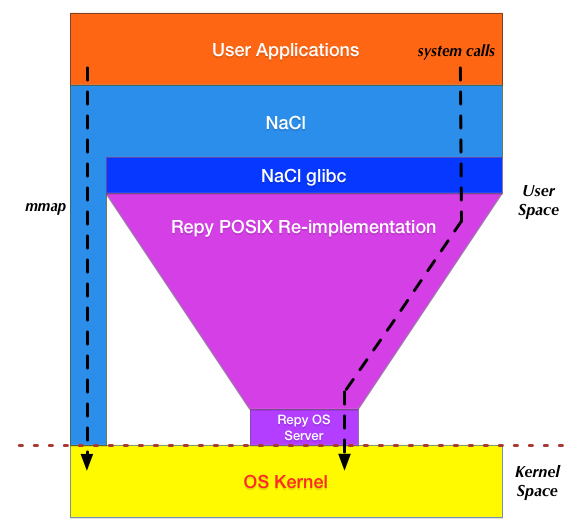
\includegraphics[width=1.0\columnwidth]{diagram/lind_architecture.png}
\caption{Architecture of Lind}
\label{fig:architecture}
\end{figure}

\subsection{Implementation Details}
Here we discuss some further implementation details about our system Lind. 
The discussion focuses mainly on the connection between the two techniques we used, 
Google's Native Client and Repy Sandbox. 

To provide native computation and safe access to the system, Lind combines NaCl and Repy. 
Untrusted programs are run in NaCl, but access to all system resources is diverted to our Repy program. 
This program is responsible for accessing the system on behalf of the program, it is called the Lind Library OS. 
Our NaCl sandbox is built on top of our Repy sandbox. To service a system call in NaCl, a server routine 
marshals its arguments into a text string, and sends the call and the arguments to Repy sandbox. 
The Library OS then executes the appropriate system call, marshals the result and returns it back to NaCl. 
The result is eventually returned as the appropriate native type to the calling program. 

Lind is designed to minimize its footprint within the trusted code base (TCB) of these two sandboxes. 
To achieve that, most of the Lind code is run from within the two sandboxes, the modifications to 
the sandboxes themselves (and therefore the TCB) was extremely small. 

The dual-layer sandbox mechanism completes the achievement of the isolation design goals through 
two features. First, the dual-layer sandbox ensures that all code can modify only device state, 
interact with devices, or interact with the outside world through the new trusted operating system interface. 
Secondly, the customizability of the interface ensures that the system can only modify state, interact with 
devices, or interact with the world at a rate and in a manner specified for the application. For example, 
any attempt to send spam or execute a denial of service attack would trigger limits on resource 
consumption and/or allowable addressing, and would be prevented. 

The dual-layer sandbox also makes the construction of Lind simpler. The complex part of Lind is the 
Library OS which runs in Repy. However, Python is a very powerful language, so it significantly simplified 
the construction of Lind. Even though Python is considered ``slow'' by some, the internals of 
an application in Lind are run in NaCl, a very high performance environment. 
This balances the performance of the system, with the ease of implementation and maintenance 
of the Library OS component of Lind. 

\cappos{Most of the rest of this isn't really central to the paper.  We 
probably should not mention it (or at least not do so prominently.}
Furthermore, this particular design and architecture for sandboxing ensures the programs are portable. 
Programs running inside Lind are written to work against a standard POSIX glibc interface. 
The Lind runtime is strictly user-level and designed to work on many different platforms including Linux, 
Mac OS X and Windows.

Our sandbox also ensures performance isolation. It is used to limit resource consumption, 
both of computational resources (CPU, memory) and external resources (disk I/O and space, 
network bandwidth). The interposed system calls rate limit access and total consumption of 
each class of device on a configurable basis. CPU and memory limits are enforced on 
a per-process basis. 

Finally, this kind of sandboxing ensures that the lightweight goal is met. Overhead for the Lind system 
is low because the sandbox only incurs overhead when there is a system call; Lind uses a native interface 
for execution, allowing CPU-and-memory-intensive applications to run at speeds that are equivalent 
to NaCl and near native speed. 

\cappos{There is an important topic shift here.  We need to signal it.}
\cappos{This also needs to be broken into multiple points / questions, I 
feel.  It is too much for a single paragraph.}
Regarding our dual-layer sandbox architecture, one fundamental question is: are two sandboxes 
enough and necessary? Why do we only have two sandboxes? If sandboxing provides more security, 
why not sandbox Repy sandbox's TCB and get more security? The answer to that question is: 
the lowest level sandbox eventually must have some fundamental yet limited access to system resources, 
such as memory, storage, threads, etc. So having multiple sandboxes is not necessary, and two sandboxes in 
our design would be enough. But are two sandboxes indeed necessary? Why not just have one sandbox 
that solves everything? The answer is that the kernel interface is extremely rich and hard to protect. 
In order to have minimal touch into the kernel, as well as provide sufficient API for legacy applications, 
we need to have more than one sandbox to complete the job. One sandbox focuses on protecting 
the kernel and providing POSIX API, the other sandbox deals with executing applications efficiently. 
That is the reason for us to have at least two sandboxes.  

\section{Evaluation}
\label{sec.evaluation}

\begin{table*}[!ht]
\begin{tabular*}{\textwidth}{l @{\extracolsep{\fill}} cccc}
\toprule
\multicolumn{5}{c}{Possibility of Triggering Kernel Vulnerabilities} \\
\midrule
Vulnerability    &  Native Linux OS  &  Lind  &  Graphene & VirtualBox\\
\midrule
 CVE-2014-9529 \cite{CVE:20149529} & \ding{55} & \ding{55} & \ding{55} & \ding{55} \\
 CVE-2014-3631 \cite{CVE:20143631} & \ding{55} & \ding{55} & \ding{55} & \ding{55} \\
 CVE-2012-6657 \cite{CVE:20126657} & \ding{55} & \ding{55} & \ding{55} & \ding{55} \\
 CVE-2014-5207 \cite{CVE:20145207} & \ding{55} & \ding{55} & \ding{55} & \ding{55} \\
 CVE-2014-5206 \cite{CVE:20145206} & \ding{55} & \ding{55} & \ding{55} & \ding{55} \\
 CVE-2014-3153 \cite{CVE:20143153} & \ding{55} & \ding{55} & \ding{55} & \ding{55} \\
 CVE-2014-2851 \cite{CVE:20142851} & \ding{55} & \ding{55} & \ding{55} & \ding{55} \\
 CVE-2014-2706 \cite{CVE:20142706} & \ding{55} & \ding{55} & \ding{55} & \ding{55} \\
 CVE-2014-0100 \cite{CVE:20140100} & \ding{55} & \ding{55} & \ding{55} & \ding{55} \\
 CVE-2014-0049 \cite{CVE:20140049} & \ding{55} & \ding{55} & \ding{55} & \ding{55} \\
 CVE-2012-6638 \cite{CVE:20126638} & \ding{55} & \ding{55} & \ding{55} & \ding{55} \\
 CVE-2014-0038 \cite{CVE:20140038} & \ding{55} & \ding{55} & \ding{55} & \ding{55} \\
 CVE-2013-6368 \cite{CVE:20136368} & \ding{55} & \ding{55} & \ding{55} & \ding{55} \\
 CVE-2013-4587 \cite{CVE:20134587} & \ding{55} & \ding{55} & \ding{55} & \ding{55} \\
 CVE-2013-4563 \cite{CVE:20134563} & \ding{55} & \ding{55} & \ding{55} & \ding{55} \\
 CVE-2013-4348 \cite{CVE:20134348} & \ding{55} & \ding{55} & \ding{55} & \ding{55} \\
 CVE-2013-4300 \cite{CVE:20134300} & \ding{55} & \ding{55} & \ding{55} & \ding{55} \\
 CVE-2013-1943 \cite{CVE:20131943} & \ding{55} & \ding{55} & \ding{55} & \ding{55} \\
 CVE-2013-2094 \cite{CVE:20132094} & \ding{55} & \ding{55} & \ding{55} & \ding{55} \\
 CVE-2013-3301 \cite{CVE:20133301} & \ding{55} & \ding{55} & \ding{55} & \ding{55} \\
 CVE-2013-1858 \cite{CVE:20131858} & \ding{55} & \ding{55} & \ding{55} & \ding{55} \\
 CVE-2013-1797 \cite{CVE:20131797} & \ding{55} & \ding{55} & \ding{55} & \ding{55} \\
 CVE-2013-1763 \cite{CVE:20131763} & \ding{55} & \ding{55} & \ding{55} & \ding{55} \\
 CVE-2013-0310 \cite{CVE:20130310} & \ding{55} & \ding{55} & \ding{55} & \ding{55} \\
 CVE-2012-2136 \cite{CVE:20122136} & \ding{55} & \ding{55} & \ding{55} & \ding{55} \\
 CVE-2012-2100 \cite{CVE:20122100} & \ding{55} & \ding{55} & \ding{55} & \ding{55} \\
 CVE-2012-0028 \cite{CVE:20120028} & \ding{55} & \ding{55} & {\color{red}\ding{51}} & {\color{red}\ding{51}} \\
 CVE-2011-2517 \cite{CVE:20112517} & \ding{55} & \ding{55} & \ding{55} & \ding{55} \\
 CVE-2012-2123 \cite{CVE:20122123} & \ding{55} & \ding{55} & \ding{55} & \ding{55} \\
 CVE-2012-1146 \cite{CVE:20121146} & \ding{55} & \ding{55} & \ding{55} & \ding{55} \\
 CVE-2012-0207 \cite{CVE:20120207} & \ding{55} & \ding{55} & \ding{55} & \ding{55} \\
 CVE-2011-2525 \cite{CVE:20112525} & \ding{55} & \ding{55} & \ding{55} & \ding{55} \\
 CVE-2011-1076 \cite{CVE:20111076} & \ding{55} & \ding{55} & \ding{55} & \ding{55} \\
 CVE-2011-2184 \cite{CVE:20112184} & \ding{55} & \ding{55} & \ding{55} & \ding{55} \\
 CVE-2010-2478 \cite{CVE:20102478} & \ding{55} & \ding{55} & \ding{55} & \ding{55} \\
 CVE-2010-2960 \cite{CVE:20102960} & \ding{55} & \ding{55} & \ding{55} & \ding{55} \\
 CVE-2010-2492 \cite{CVE:20102492} & \ding{55} & \ding{55} & \ding{55} & \ding{55} \\
 CVE-2010-2240 \cite{CVE:20102240} & {\color{red}\ding{51}} & \ding{55}  & {\color{red}\ding{51}} & {\color{red}\ding{51}} \\
 CVE-2010-1188 \cite{CVE:20101188} & \ding{55} & \ding{55} & \ding{55} & \ding{55} \\
 CVE-2010-0437 \cite{CVE:20100437} & \ding{55} & \ding{55} & \ding{55} & \ding{55} \\
\bottomrule
\end{tabular*}
\caption {Possibility of Triggering Kernel Vulnerabilities 
({\color{red}\ding{51}}: possible to trigger the bug; \ding{55}: not possible to trigger the bug)
{\color{red}(The results are fake at the moment)}}
\label{table:trigger_vulnerabilities}
\end{table*}

\subsection{Evaluation Methodology}
We want to evaluate our metric, and new architecture and designs that came from our metric. 
The methodology is we implement one new system Lind, using our new design, and compare it 
with other systems not using our design. The comparison results will show if our system is better, 
which in turn will show if our metric is effective. 

We conducted comparison between Lind and other systems, which were Native Linux, 
VirtualBox and Graphene. Native Linux was used as a baseline, while VirtualBox and Graphene
were both competitive systems that also aimed at user application isolation.

In order to conduct the comparison, we first generated the kernel trace from each of the different 
environments. We used system call fuzzing and popular user applications to generate the kernel trace. 

\subsection{The Comparison Results and Analysis}
Our primary goal is to build a secure system. Therefore, our core evaluation is for the security aspect. 
We also did performance evaluation to show that our system Lind has reasonable performance overhead, 
which is not our focus. 

\subsubsection{Security Evaluation}
Since Lind aims at achieving a very secure system, and leverages our metric by using its 
security-prioritized guidelines. We first focused on comparing the security of each of the systems.

Again, we used two approaches, system call fuzzing and running user applications, to obtain the
kernel profiling data. 

We first compared the kernel trace under different environments.
The comparison results for running system call fuzzing and user applications in different systems 
are shown in Figure 4 and 5.

From Figure 4 and Figure 5, we can see that the kernel trace of Lind has significant overlap with that of Native Linux, 
which shows that Lind triggered most of the commonly used kernel paths that are safe. And when comparing 
with VirtualBox and Graphene, both systems have very huge different trace from Lind, which shows VirtualBox and Graphene
used a lot of kernel paths other than commonly used kernel paths, which may contain more bugs.  

\begin{figure}[h]
\centering
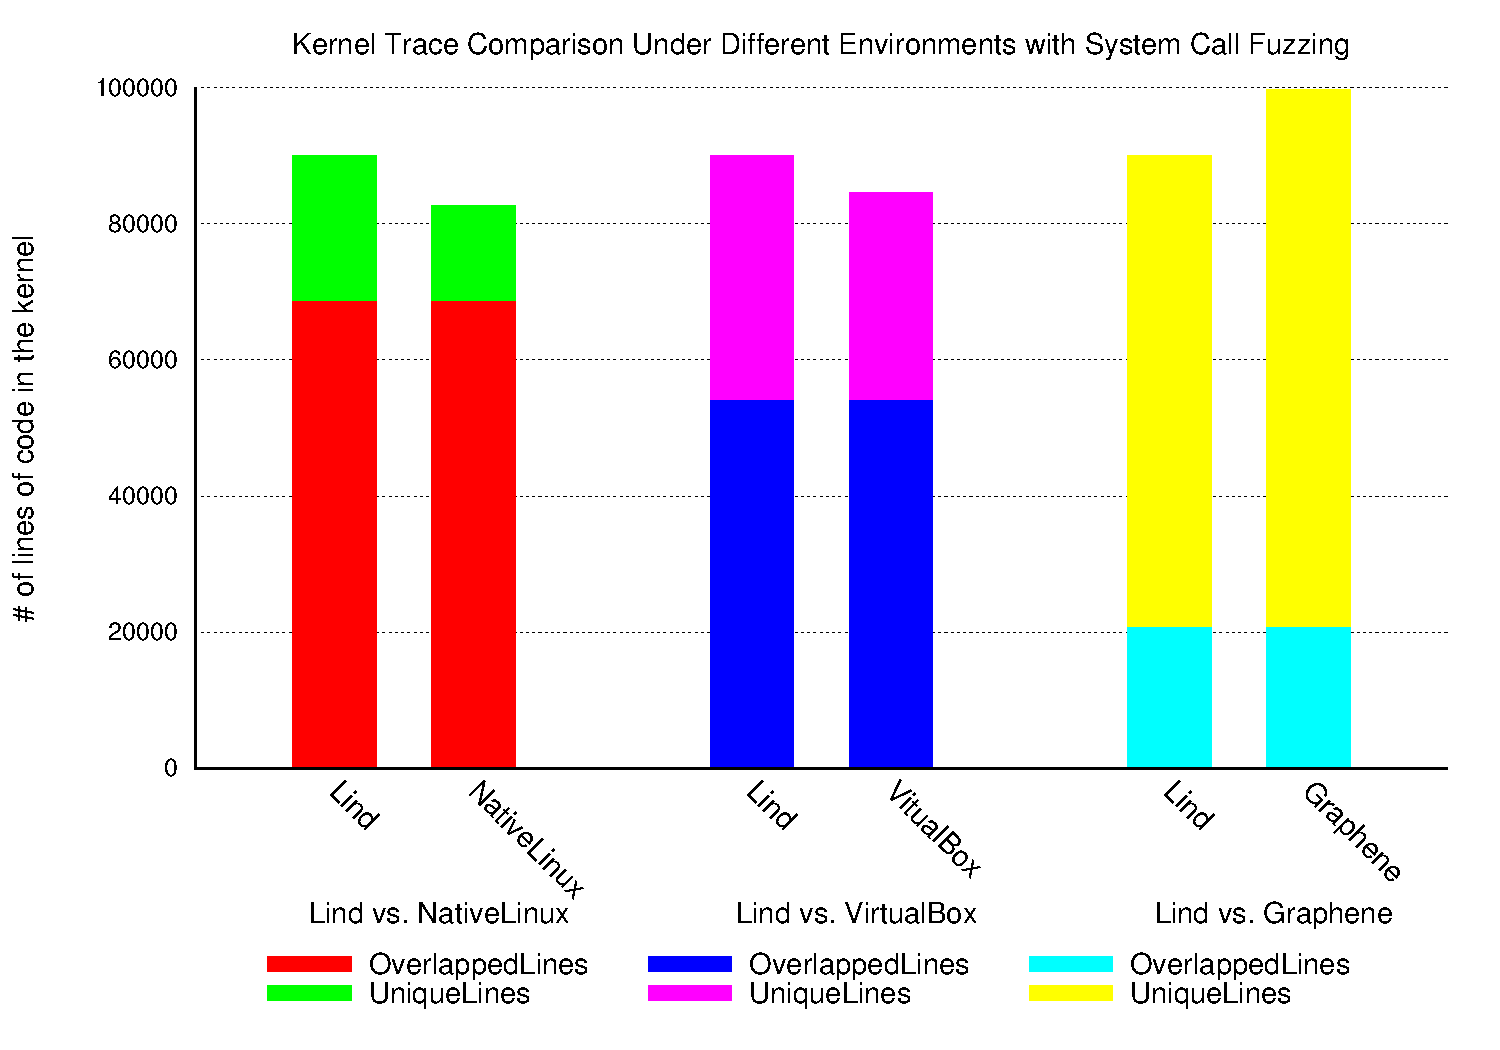
\includegraphics[width=1.0\columnwidth]{diagram/lind_ccs15_diagram_03.pdf}
\caption{Kernel Trace in Different Systems with System Call Fuzzing {\color{red}(The results are fake at the moment)} }
\label{fig:different_systems_systemcallfuzzing_trace}
\end{figure}

\begin{figure}[h]
\centering
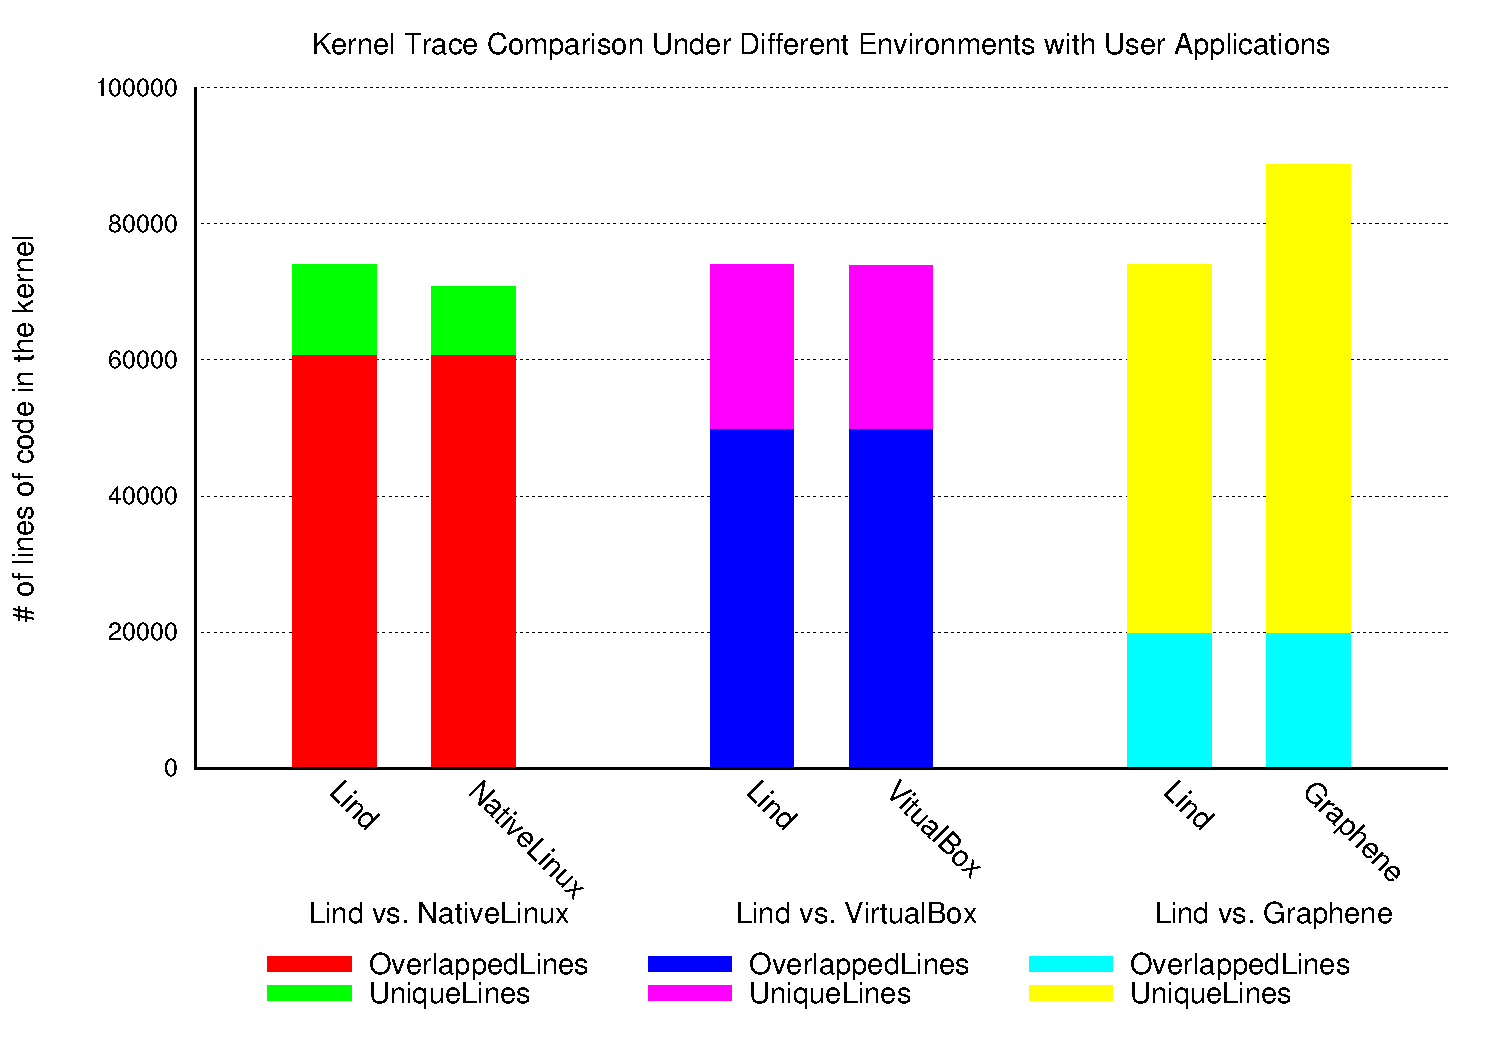
\includegraphics[width=1.0\columnwidth]{diagram/lind_ccs15_diagram_04.pdf}
\caption{Kernel Trace in Different Systems with Running User Applications {\color{red}(The results are fake at the moment)}}
\label{fig:different_systems_userapplications_trace}
\end{figure}

Now, we want to verify how likely it is to trigger kernel bugs in each of the environment.
We already had kernel trace generated by running system call fuzzing and user applications.
In order to check if kernel bugs might appear in those traces, we examined a list of 40 severe Linux 
kernel bugs (shown in Table 1), and identified the kernel paths involved in triggering each of the bugs.

The list of bugs we used in our experiments is shown in Table 1.

After examination of the bugs, we matched the kernel traces in different environments against the kernel traces generated 
by the bugs to verify if a bug might be triggered under each environment. 

The results for verifying which kernel bugs may be triggered under each environment is illustrated in Table 4.
From the results, we can see that Lind tends to provide stronger security than other systems.  

\subsubsection{Performance Evaluation}
Besides the security evaluation, we also did performance evaluation on running applications in each of the different environments.
The purpose of this performance evaluation is to show that although system like Lind is designed and built to provide stronger
security, it can also function well with reasonable overhead. 

Comparison results for the performance evaluation are shown in Figure 6.
The results show that the overhead of running applications in Lind is acceptable, compared with other systems. 
This suggests that systems designed and built using our metric can achieve the design goals, as well as function well in practice. 

\begin{figure}[h]
\centering
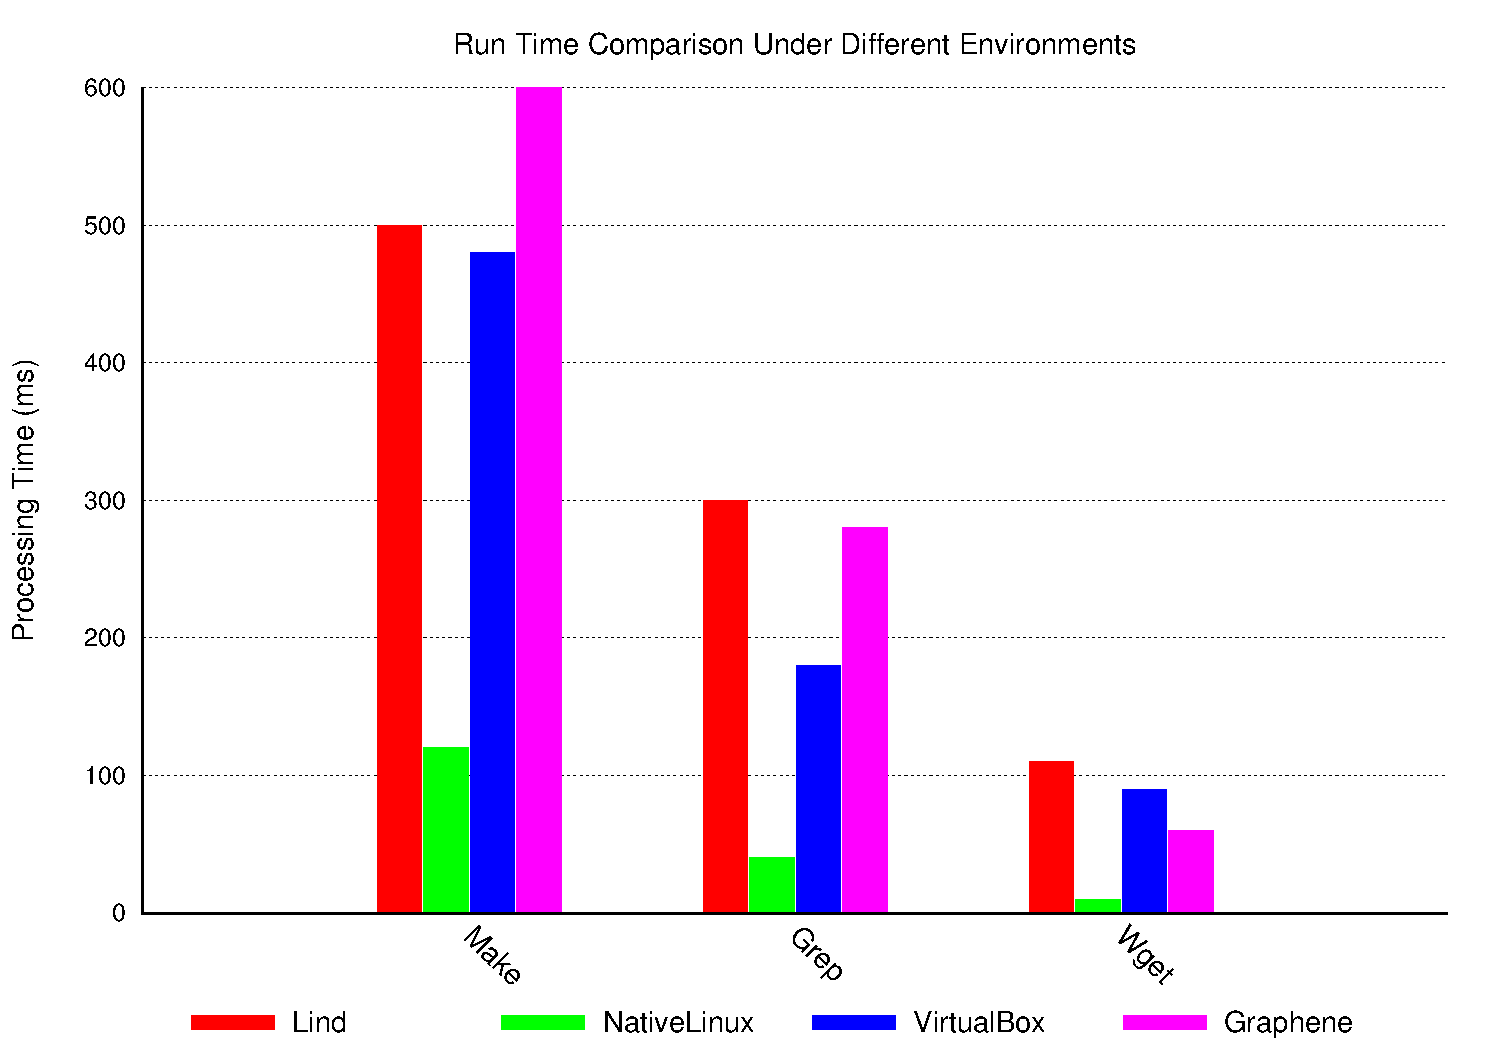
\includegraphics[width=1.0\columnwidth]{diagram/lind_ccs15_diagram_05.pdf}
\caption{Performance Evaluation Results {\color{red}(The results are fake at the moment)}}
\label{fig:performance_evaluation_results}
\end{figure}

\subsection{Conclusion}
Through our security evaluation and performance evaluation, we can see that 
Lind indeed achieved stronger security, compared against other systems.
Our metric is effective in creating new designs for building secure systems. 
\section{Related Work}
\label{sec.related_work}

Many previous ideas and systems have helped and inspired us. We categorize and discuss closely related work below.

\cappos{Given the organization of the paper, I'm not sure if other software 
engineering techniques to find bugs fit in here too.  For example, the FixCache
work and follow on papers.  I would be tempted to put them in
the early sections instead, but I haven't really thought about it much.}

\subsection{Measuring and Profiling the Kernel}

To our best knowledge, our proposed metric is the first quantitative metric to profile the kernel trace. 
There are other work that tried to measure and profile the kernel. However, their goals and approaches 
had substantial differences from ours.
\yiwen{I need to add related work in this area and briefly discuss the differences
between their approaches and ours.} 


\subsection{Historical Kernel Bug Analysis}
Historical kernel bug reports indicate the vulnerabilities hidden in the kernel space. 
Previous work has studied many of the historical kernel bugs and gathered statistics. 
However, there has yet to be any concrete method to match any specific kernel bug to the kernel code.  
Our metric could fill in the gap and leverage kernel bug reports to help new system designs more effectively.
\yiwen{More related work needs to be added.}

\subsection{Isolation Between the Kernel Space and the User Space}

As an instantiation of new designs using our metric, our sandbox system Lind aims at building a highly secure system 
that provides strong isolation between the kernel space and the user space. Many existing techniques also tried to 
address security issues by isolating the kernel space and the user space. In this section, we look closely into the techniques 
that share similar security goals as Lind. We further categorize those techniques into three categories and discuss them 
in \S{7.3.1}, \S{7.3.2}, and \S{7.3.3}. 

\subsubsection{Virtualization}

Programming language virtualization, such as Java, Silverlight, JavaScript and Flash are commonly used sandboxes that 
have achieved widespread adoption. These sandboxes combine untrusted application code with an interpreter and 
standard libraries. Standard libraries consolidate routines to perform I/O, network communication, and other system sensitive 
functionality. Though many sandboxes implement the bulk of their standard libraries in a memory-safe language like 
Java or C\#, flaws in memory-safe code can still pose a threat.

Virtualization is widely used to isolate untrusted applications that share the same hardware. There is bare metal hardware 
virtualization, such as VMware ESX Server, XEN \cite{Xen:03}, and MS Hyper-V. There is also hosted hardware virtualization, 
such as VMware Workstation, VMware Server, MS Virtual PC and Server. However, there are limitations with virtualization. 
Virtualization hypervisor suffers from attack vectors including architectural vulnerability, software vulnerability, 
and configuration risk. For example, small code footprint of hypervisor could become a potential vulnerability 
and lead to serious problem.

Drawbridge \cite{Drawbridge:11} uses light-weight processes and a library OS to present a Windows persona to 
a wide variety of Windows applications. This is accomplished by moving a large portion of the OS into the process, 
and presenting a simplified system virtual machine like interface to each process. This approach brings many of 
the benefits of VM based temporal, spatial and fault isolation properties to a per-process level.


\subsubsection{System Call Interposition}

System call interposition offers a number of properties that make it attractive for building sandboxes, 
though it can be error prone \cite{SCI:04}. Approaches for delegation and filtering have been extensively studied, 
along with their respective tradeoffs with security and performance. Janus Version 2 (J2) \cite{Janus0:96, Janus:99} 
uses filtering and sandboxing, while Ostia \cite{SCI:04} uses a delegation.

Ostia also provides a hybrid interposition architecture, which allows for kernel level enforcement and user policies. 
The Kernel module enforces policy, denies direct access to restricted resources, and delegates certain calls to 
the Emulation library, which sends transformed system calls to the Agents. The Agent reads the policy file and 
handles the delegation of calls.


\subsubsection{Software Fault Isolation}

Software Fault Isolation (SFI) is a sandboxing technique in which native instructions are executed, but only those instructions 
which can be executed without violating the sandbox's constraints are allowed \cite{SFI:93}. Instructions usually excludes 
are those which could jump outside the program's predefined memory region or execute a system call. 
Programs must use a specific compiler which enforces these constraints, then the programs are validated on load. 
Nooks \cite{Nooks:03} isolates Linux kernel modules, so that when they crash the whole kernel does not crash as well. 
They use two techniques: sandboxing and micro-reboots. Nooks uses both as SFI-based and user-level sandbox. 
Micros-reboots conceptually refresh small parts of the system.

\section{Conclusion}
\label{sec.conclusion}

\cappos{I feel we will really need a limitations section.  It's clear there
are a lot of things we could do to round out the work.  For example,
using other OSes for analysis (Windows, etc.), testing hypervisors, etc.
I do not know if it can be a subsection here, but it is worth being
very direct about. }

\cappos{On a similar note, we likely also need to be very clear about the
limitations / framing of the problem up front so the reader does not expect
more than we provide.}

Isolating untrusted user applications from the underlying kernel is
desirable, in order to protect the privileged code and 
avoid the exploitation of bugs. However, there has yet to be a standard
method that can shed lights on how to effectively
isolate the user space applications from the kernel space without losing
desired functionality.

We propose a new metric that quantitatively measures and evaluates the
kernel code being executed when running
user applications. We have a key hypothesis that commonly used kernel paths
contain few bugs. Using our metric, 
we have findings suggesting the hypothesis is reasonable and solid. 

A new design for building secure systems was created based on the findings
from our metric. 
We implemented a sandbox system, called Lind, which is based upon the new
design using our metric. 
Our system Lind, securely reconstruct complex yet essential OS
functionality inside a sandbox. 
The sandbox itself is designed to have a minimized trusted computing base
(TCB) and only interact with the kernel
in a minimal and safe way. 

Our evaluation results have shown that Lind is least likely to trigger
historically reported kernel bugs, compared against
other systems built without using our metric, such as VirtualBox and
Graphene. The successful implementation of Lind
suggests that new designs using our metric are likely to lead to more
secure systems. 


%%%%%%%%%%%%%%%%%%%%%%%%%%%%%%%%%%%%%%%%%%%
%  Bibliography
%%%%%%%%%%%%%%%%%%%%%%%%%%%%%%%%%%%%%%%%%%%

\bibliographystyle{abbrv}
\bibliography{paper}

%%%%%%%%%%%%%%%%%%%%%%%%%%%%%%%%%%%%%%%%%%%
%  End of Document
%%%%%%%%%%%%%%%%%%%%%%%%%%%%%%%%%%%%%%%%%%%

\end{document}